\section{Megvalósítás}
\subsection{Használt erőforrások}
A háló összerakást saját gépen kezdtük el. Majd a véglegesítését és a tanításokat AWS szerveren, NVIDIA Tesla K80 12GB videokártyán végeztük. Jupyter notebook-ban futtatuk a tanításokat, ezek elmentett adatait aztán Tensorboard segítségével elemeztük.

\subsection{Eredmények}
\subsubsection{Zöngésség}
Zöngésség becslésére nagyon jó, alapfrekvencia (pitch érték) meghatározására használhatóan jó és a spektrális paraméter (Mel-Cepstrum) jósolására kezdetleges eredményeket sikerült elérnünk. (utóbbiról ezért nem is mellékeltünk tanítási és validációs grafikonokat). Hiperparaméter optimalizálás tekintetében egyelőre kézzel dolgoztunk (ez még javításra szorul), már így is sikerült használható pontosságot  elérnünk.

\textit{(A grafikonk y tengelyén az MSE hiba értéke x tengelyén az elvégzett epoch-ok száma látható.)}

\begin{minipage}{0.5\textwidth}
	Zöngésség becslése egyszerűbb, futásidő tekintetében gyorsabb feladatnak bizonyult. Ezért itt nem alkalmaztunk early stopping-ot, hanem a több próbálkozás után a fixen 410 epoch-kal történő tanításnál maradtunk.
	
	A teszt adatainkon elért eredmények:
	
	pontosság 0.8342
	
	költségfüggvény: 0.1560
	
	\textit{(MSE hiba értékekkel számítva)}
\end{minipage}
\begin{minipage}{0.5\textwidth}
	\flushright	
	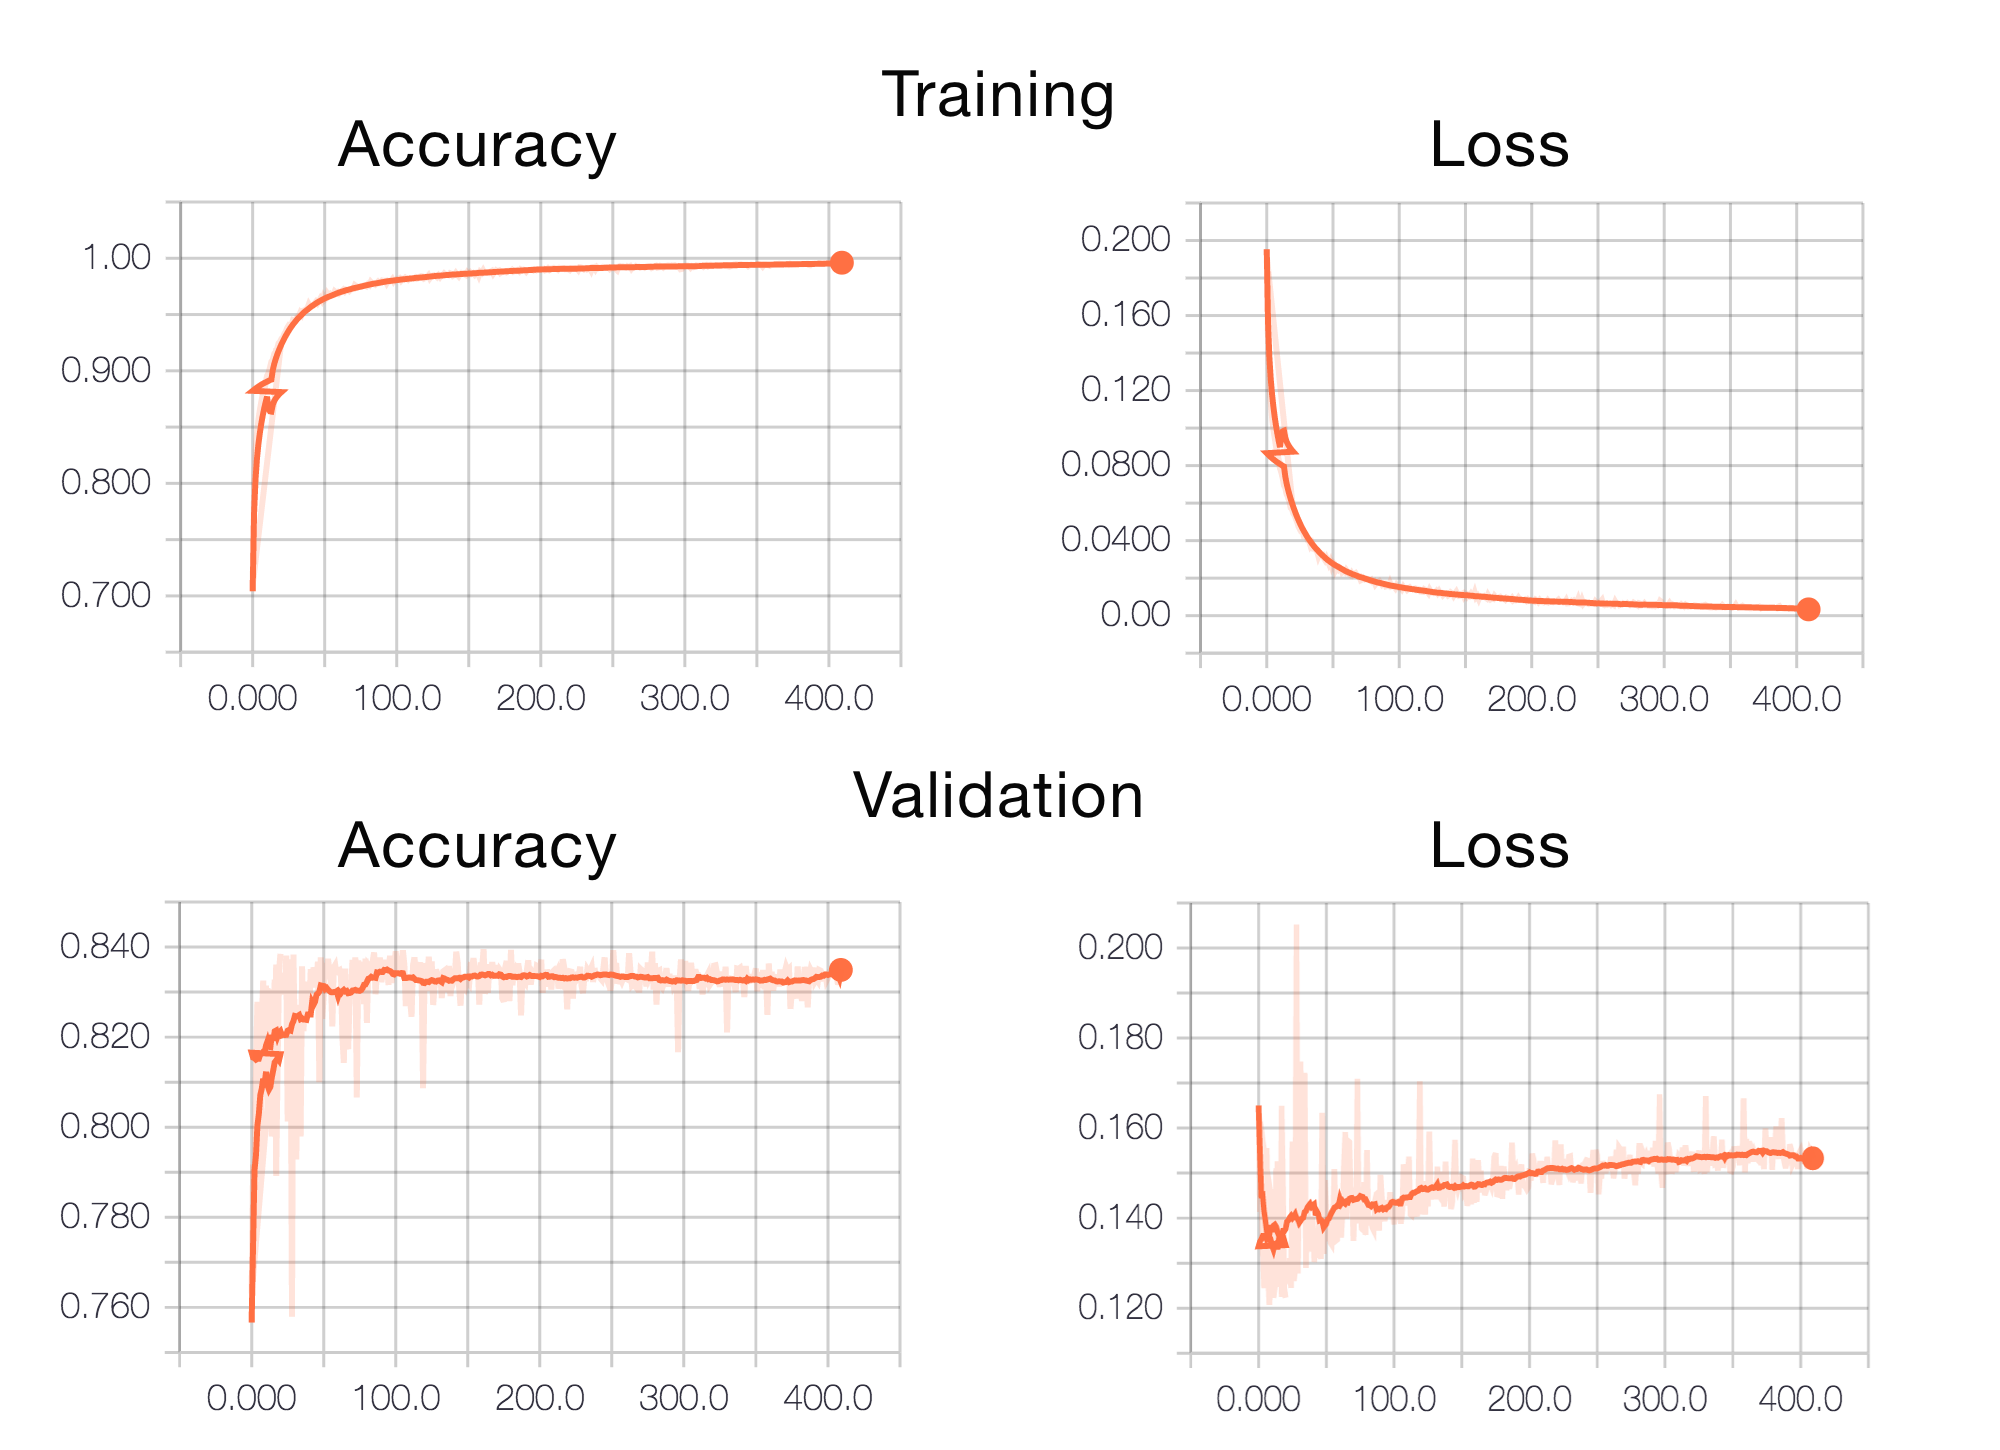
\includegraphics[width=0.8\textwidth,keepaspectratio]{uv_fig}
\end{minipage}
\subsubsection{Alapfrekvencia}
Az alapfrekvencia tanítása esetén alkalmaztunk early stoppig-ot. Ez azonban (a paramétereinek állítása után is) túl hamar állt meg. Ennek következtében több tanítást is elvégeztünk egymás után. Az itt kapott eredményeink messze nem olyan szépek mint a zöngésségé, de ezek is használhatónak bizonyultak.

A teszt adatainkon elért eredmények:

pontosság: 0.4243

költségfüggvény: 0.07214

\textit{(MSE hiba értékekkel számítva)}

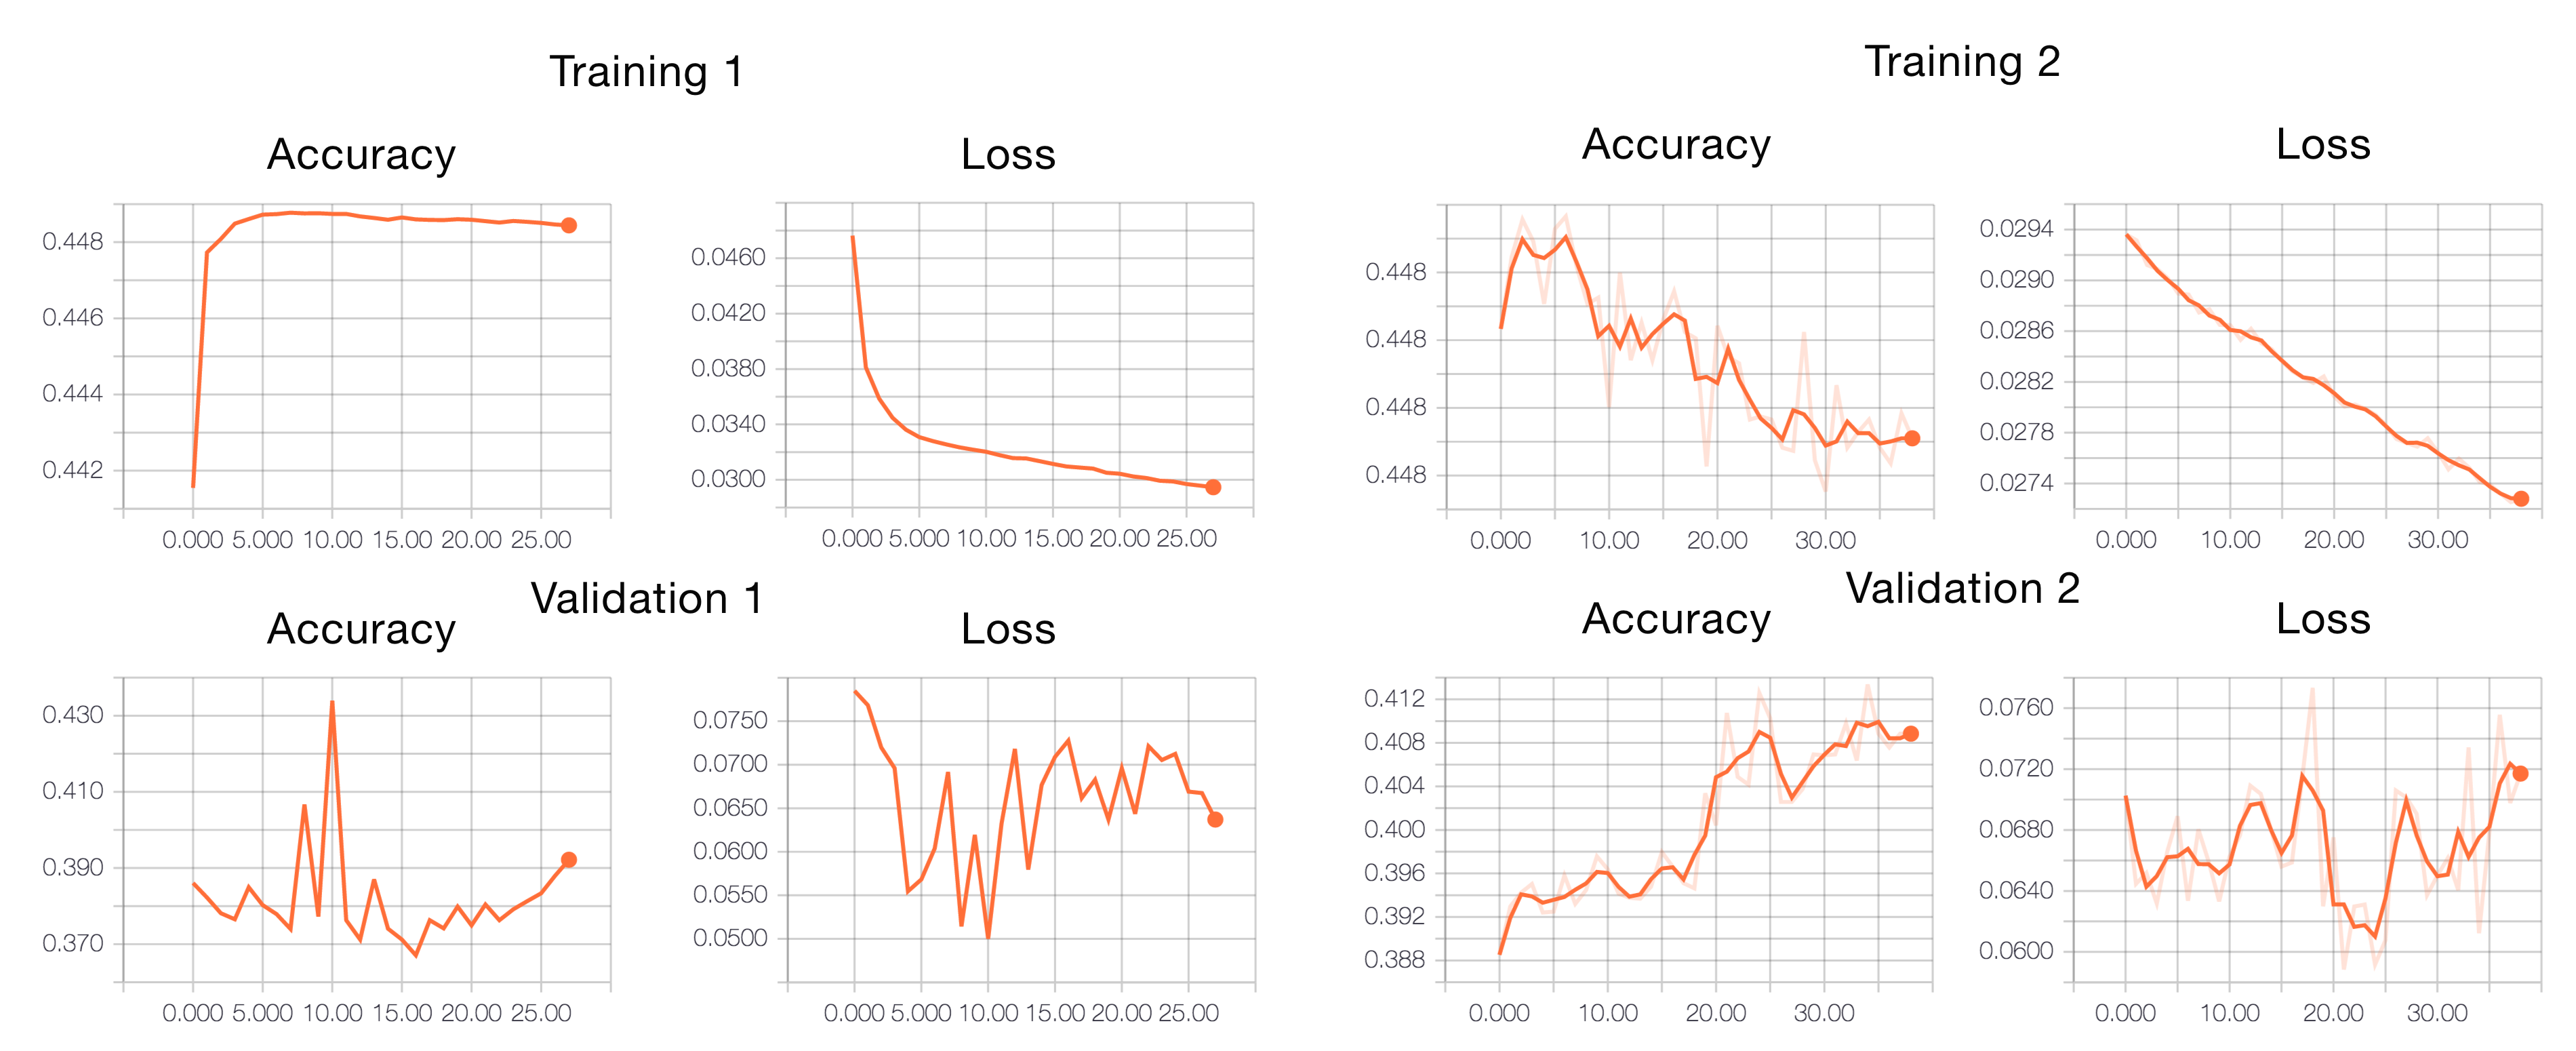
\includegraphics[width=\textwidth,keepaspectratio]{pitch_fig}
\subsubsection{MC paraméterek}
MC tanításakor kiütközött, hogy a bemeneti paramétereink nagyon megegyezőek voltak fonémán belül, így darabos lett a tanítás. Ez a magasabb MC értékekre jelentős hibát okozott, így megpróbáltuk kevesebb mc érték használatát pontosítani.

\begin{minipage}{0.5\textwidth}	
	A teszt adatainkon elért eredmények:
	
	pontosság 0.2927
	
	költségfüggvény: 0.2086
	
	\textit{(MSE hiba értékekkel számítva)}
\end{minipage}
\begin{minipage}{0.5\textwidth}
	\flushright	
	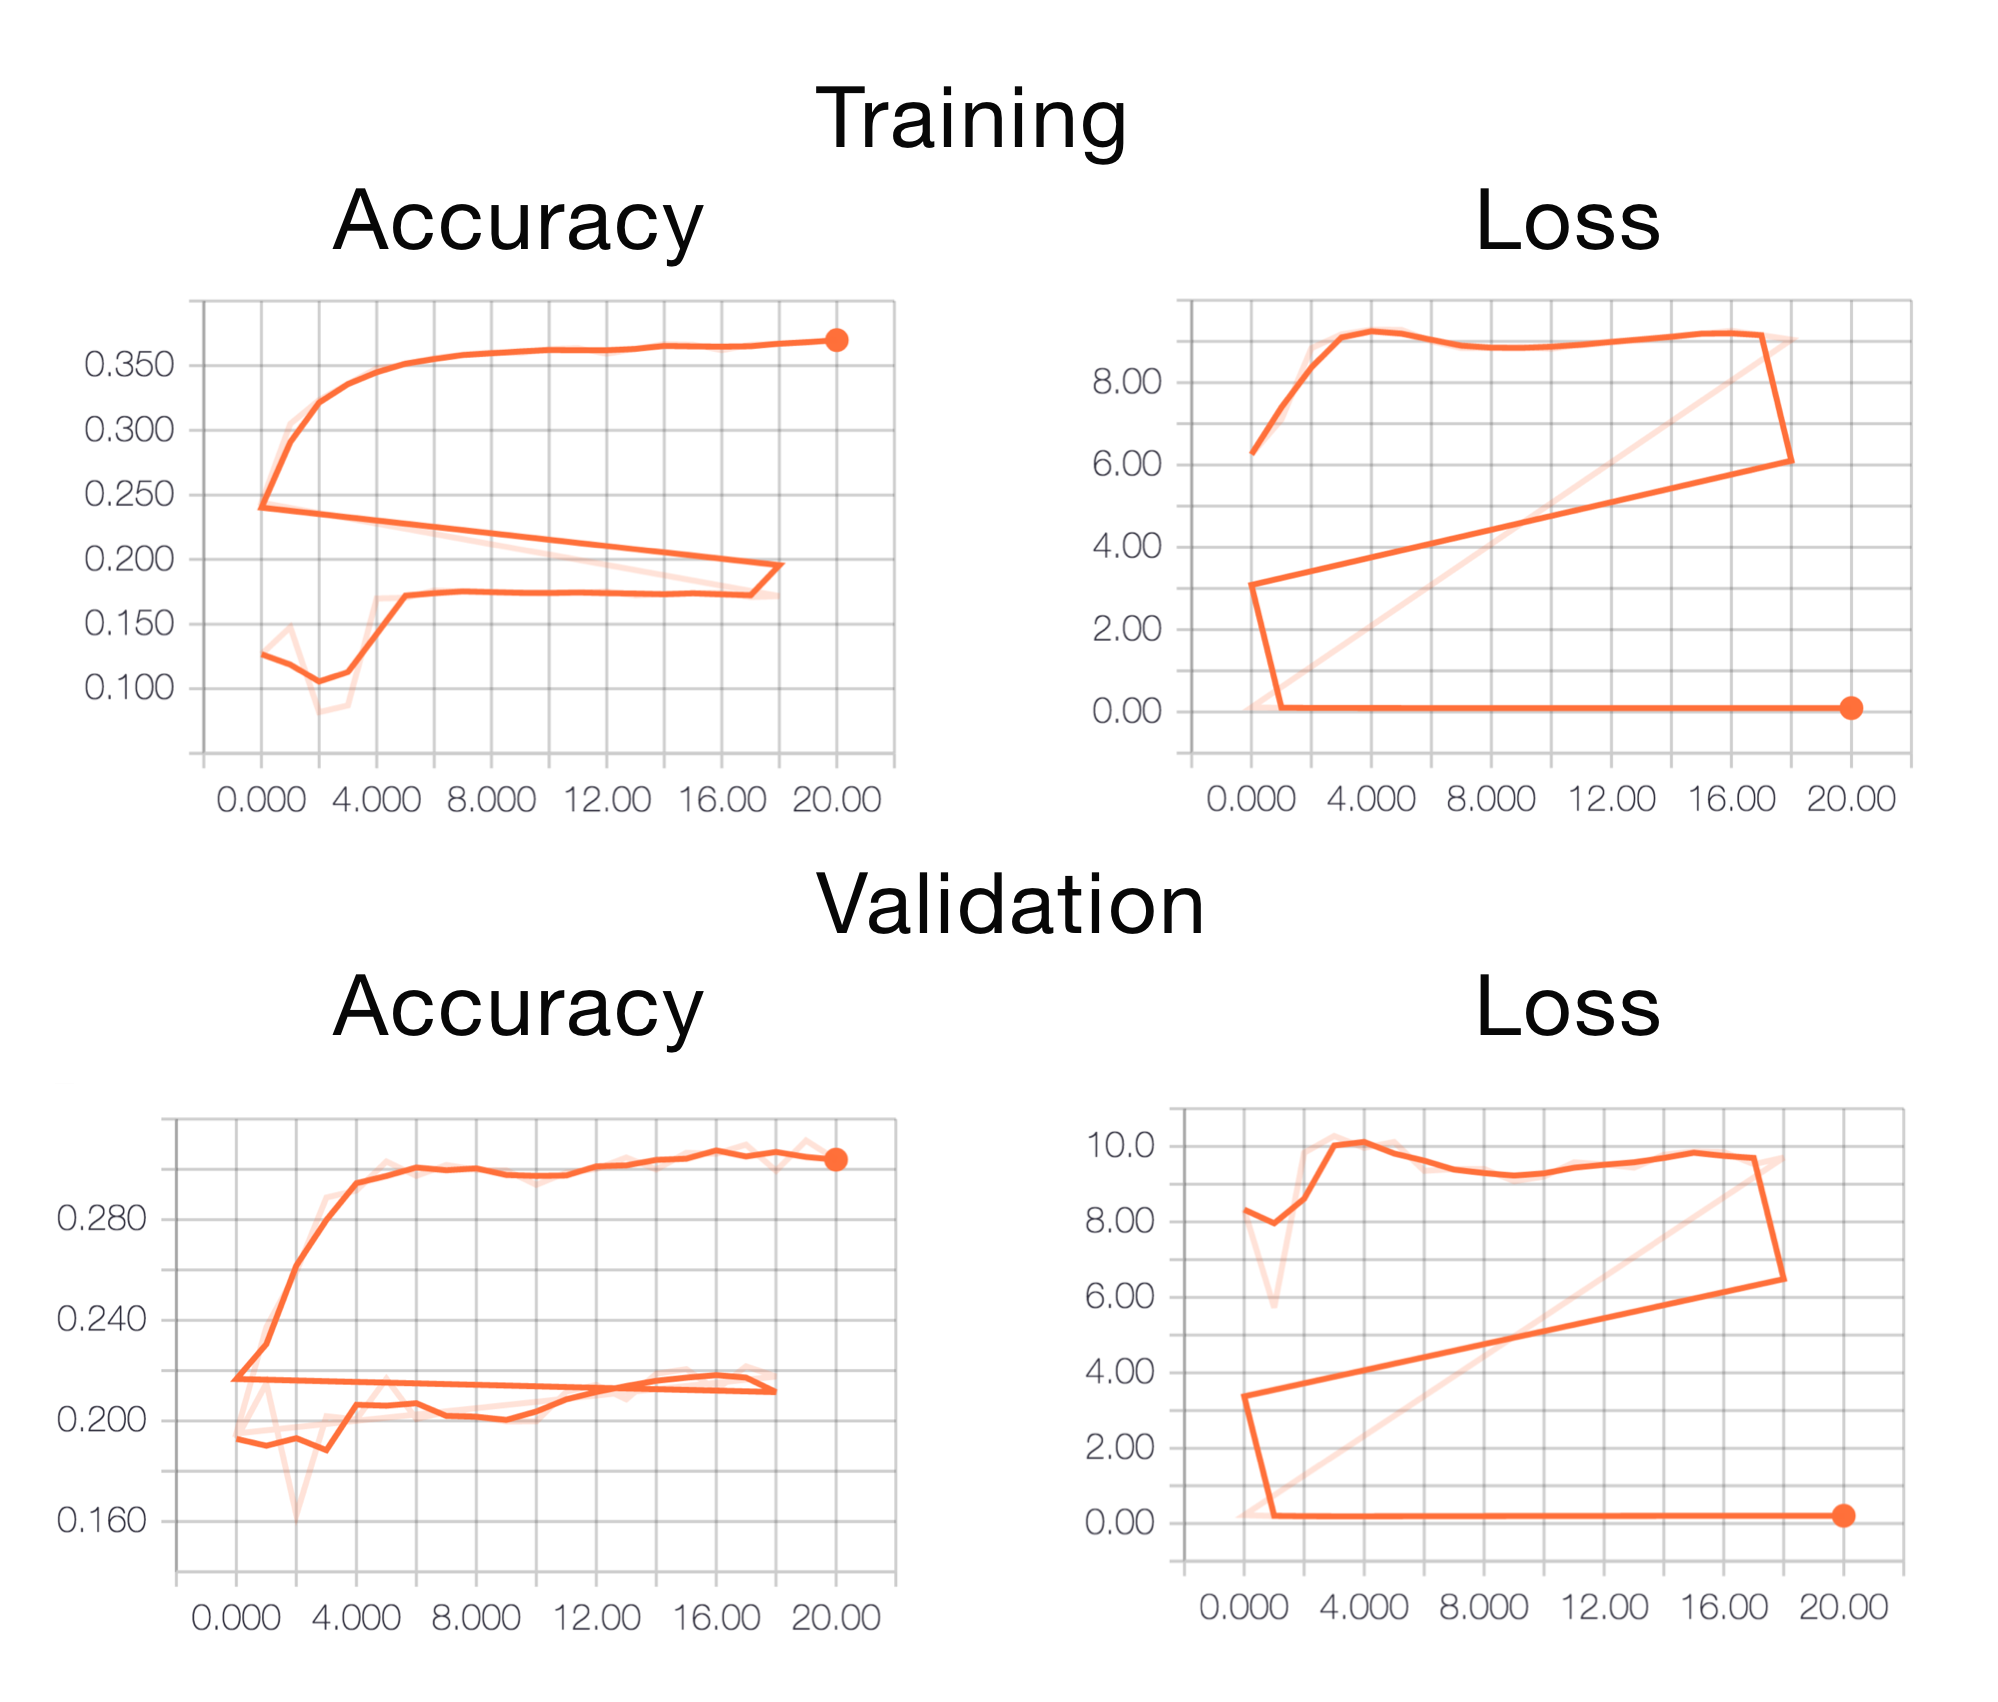
\includegraphics[width=\textwidth,keepaspectratio]{length_fig}
\end{minipage}
\subsubsection{Fonéma hossz}
Fonéma hossz becslésnél csoportosítást valósítottunk meg, a fonémákat 8 csoportba osztottuk, a csoportok között 12,5 ms eltéréssel és a csoportra végeztünk classificationt. Erre azért volt szükség mivel viszonylag kevés, géppel annotált tanító adat állt a rendelkezésünkre, ezek alapján nem sikerült használható eredményeket elérni. Az adatokban szereplő eredeti hosszak vizsgálata után ezt a csoportosítási módot választottuk, két szempont a megfelelő differenciálódás és a jelentősen kilógó adatok levágása volt. Tehát minden fonémánk 40 és 140 ms közé került. (A tanító adatainkat is ez alapján módosítottuk még a feldolgozási fázisban, minden keretnél hosszabb fonémát 140 ms-nél levágunk.)

\begin{minipage}{0.5\textwidth}	
	A teszt adatainkon elért eredmények:
	
	pontosság 0.4619
	
	költségfüggvény: 0.02419
	
	\textit{(MSE hiba értékekkel számítva)}
\end{minipage}
\begin{minipage}{0.5\textwidth}
	\flushright	
	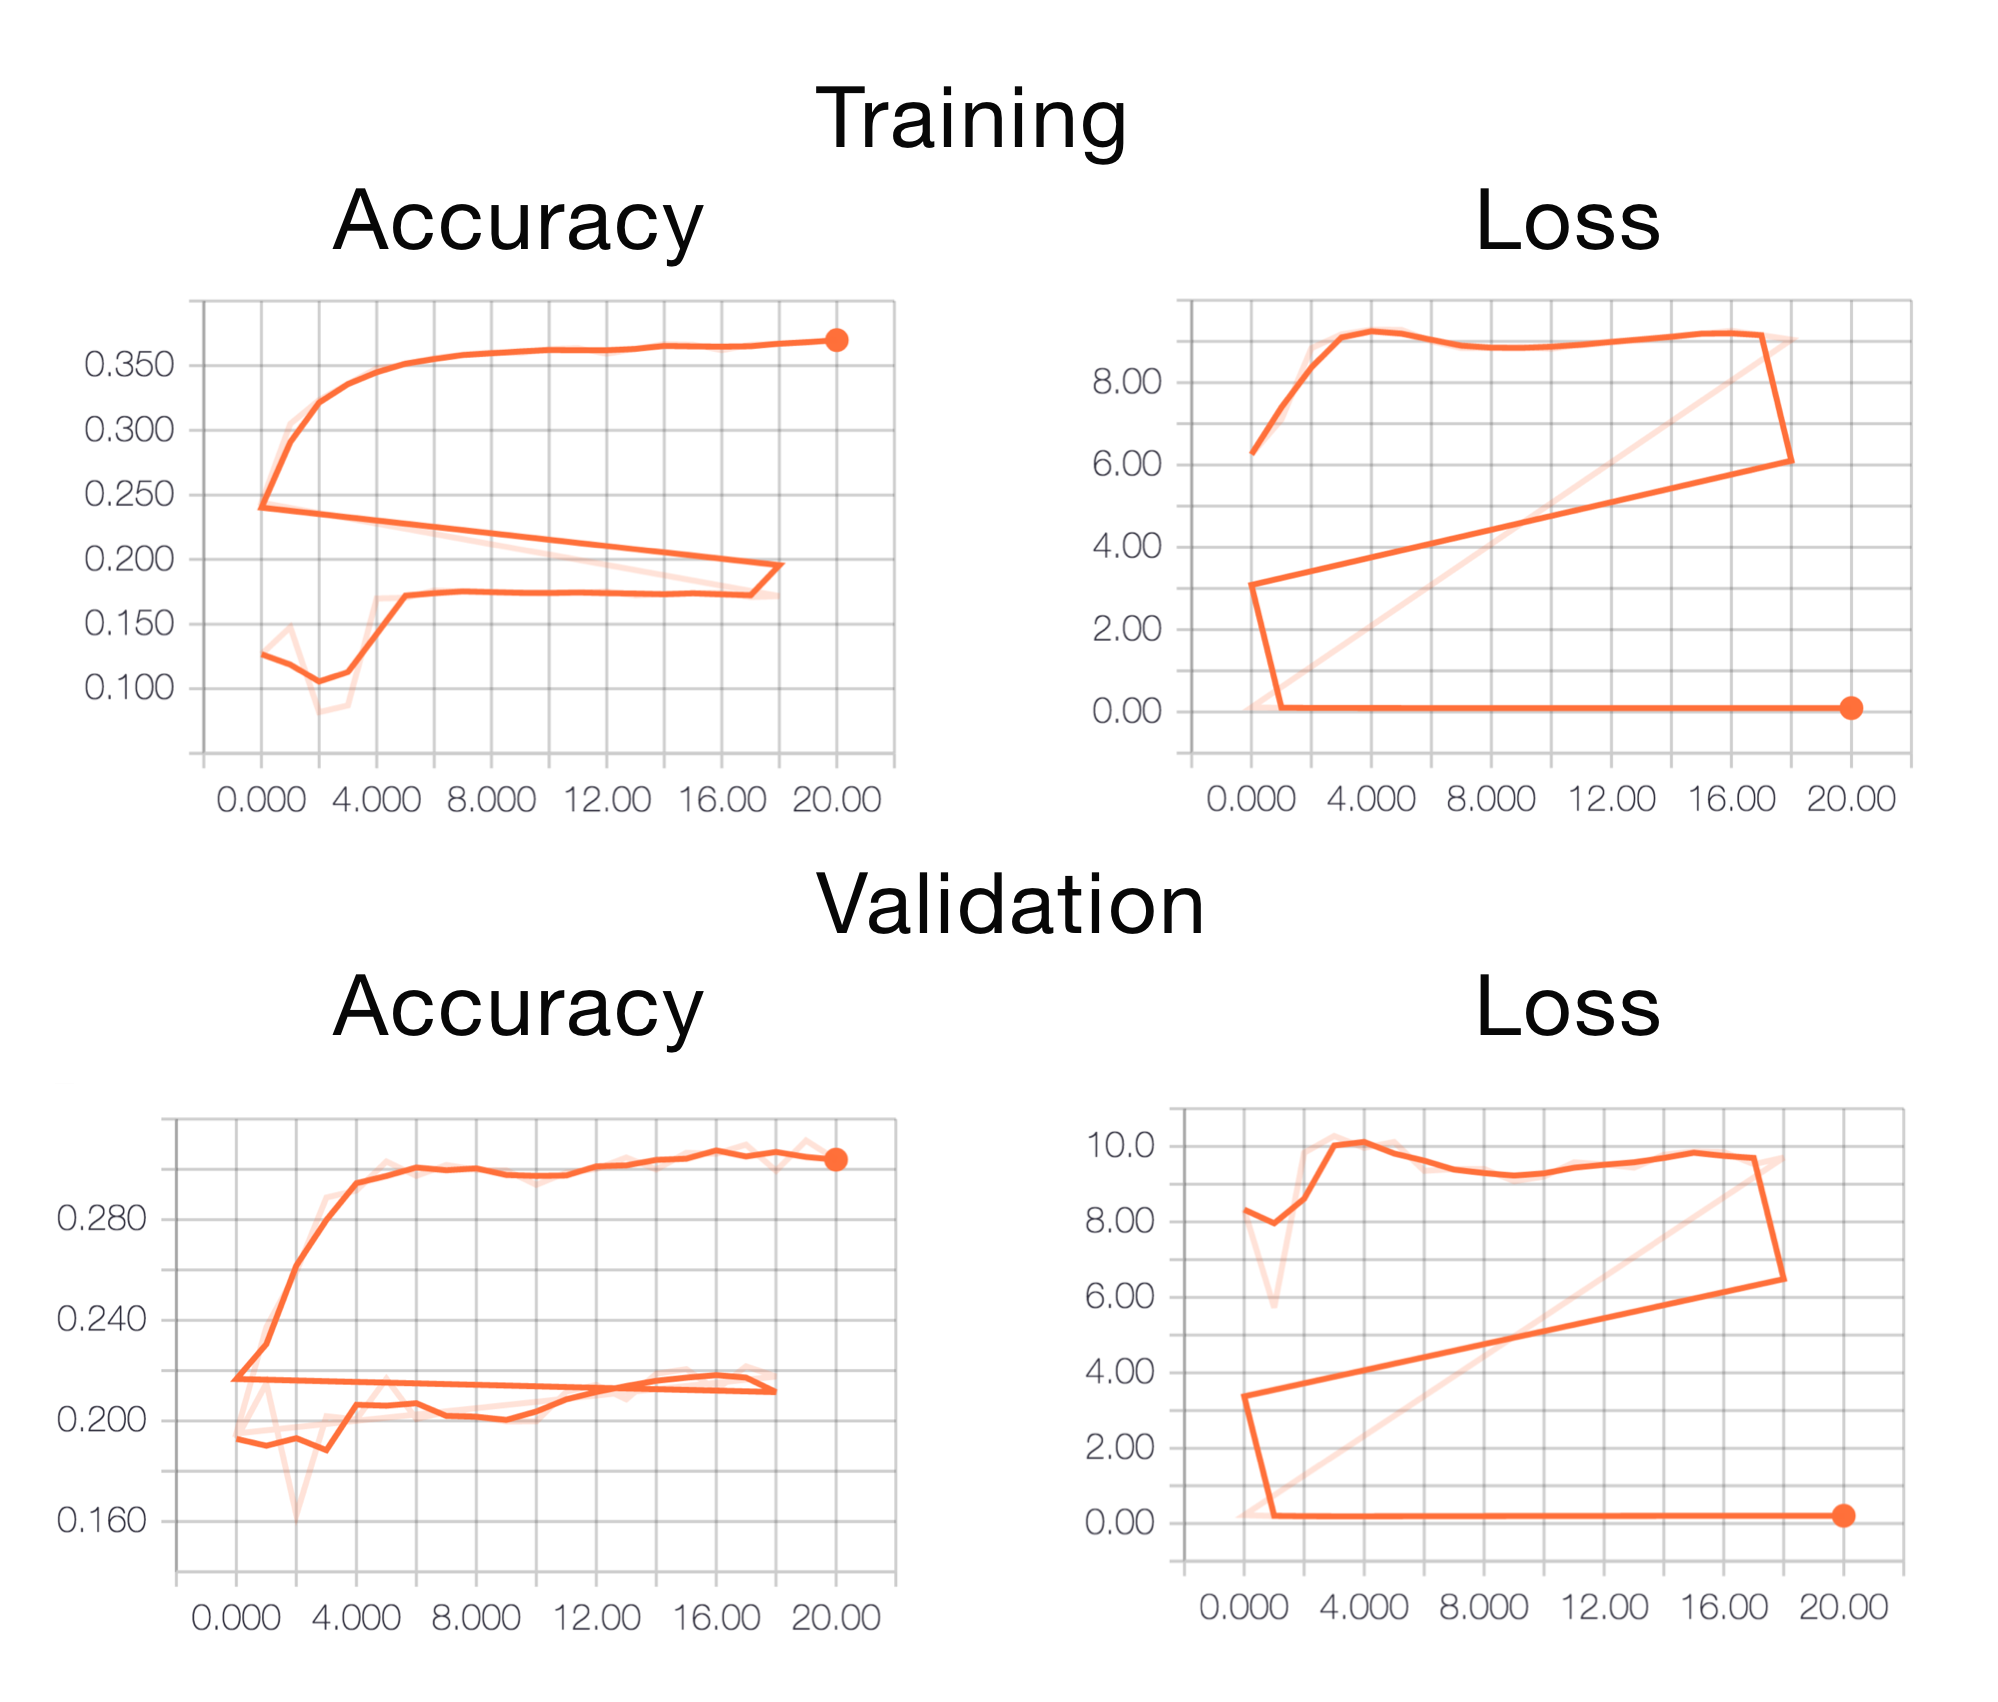
\includegraphics[width=\textwidth,keepaspectratio]{length_fig}
\end{minipage}

\subsubsection{Teljes becslő}
A fenti paraméterek ismeretében teljes TTS végezhető. 

A mondat alapján fonéma hosszakat becslünk, majd párhuzamosan zöngésség-alapfrekvencia és mc paraméter becslés folyik, végül a kapott eredményekből előállítható a kimenet.